\section{Programación Genética}

\subsection{Como funciona Programación Genética}

Programación Genética es un tipo de algoritmo evolutivo.

\subsubsection{Bases de algoritmos evolutivos}

\begin{figure}[H]
    \centering
	  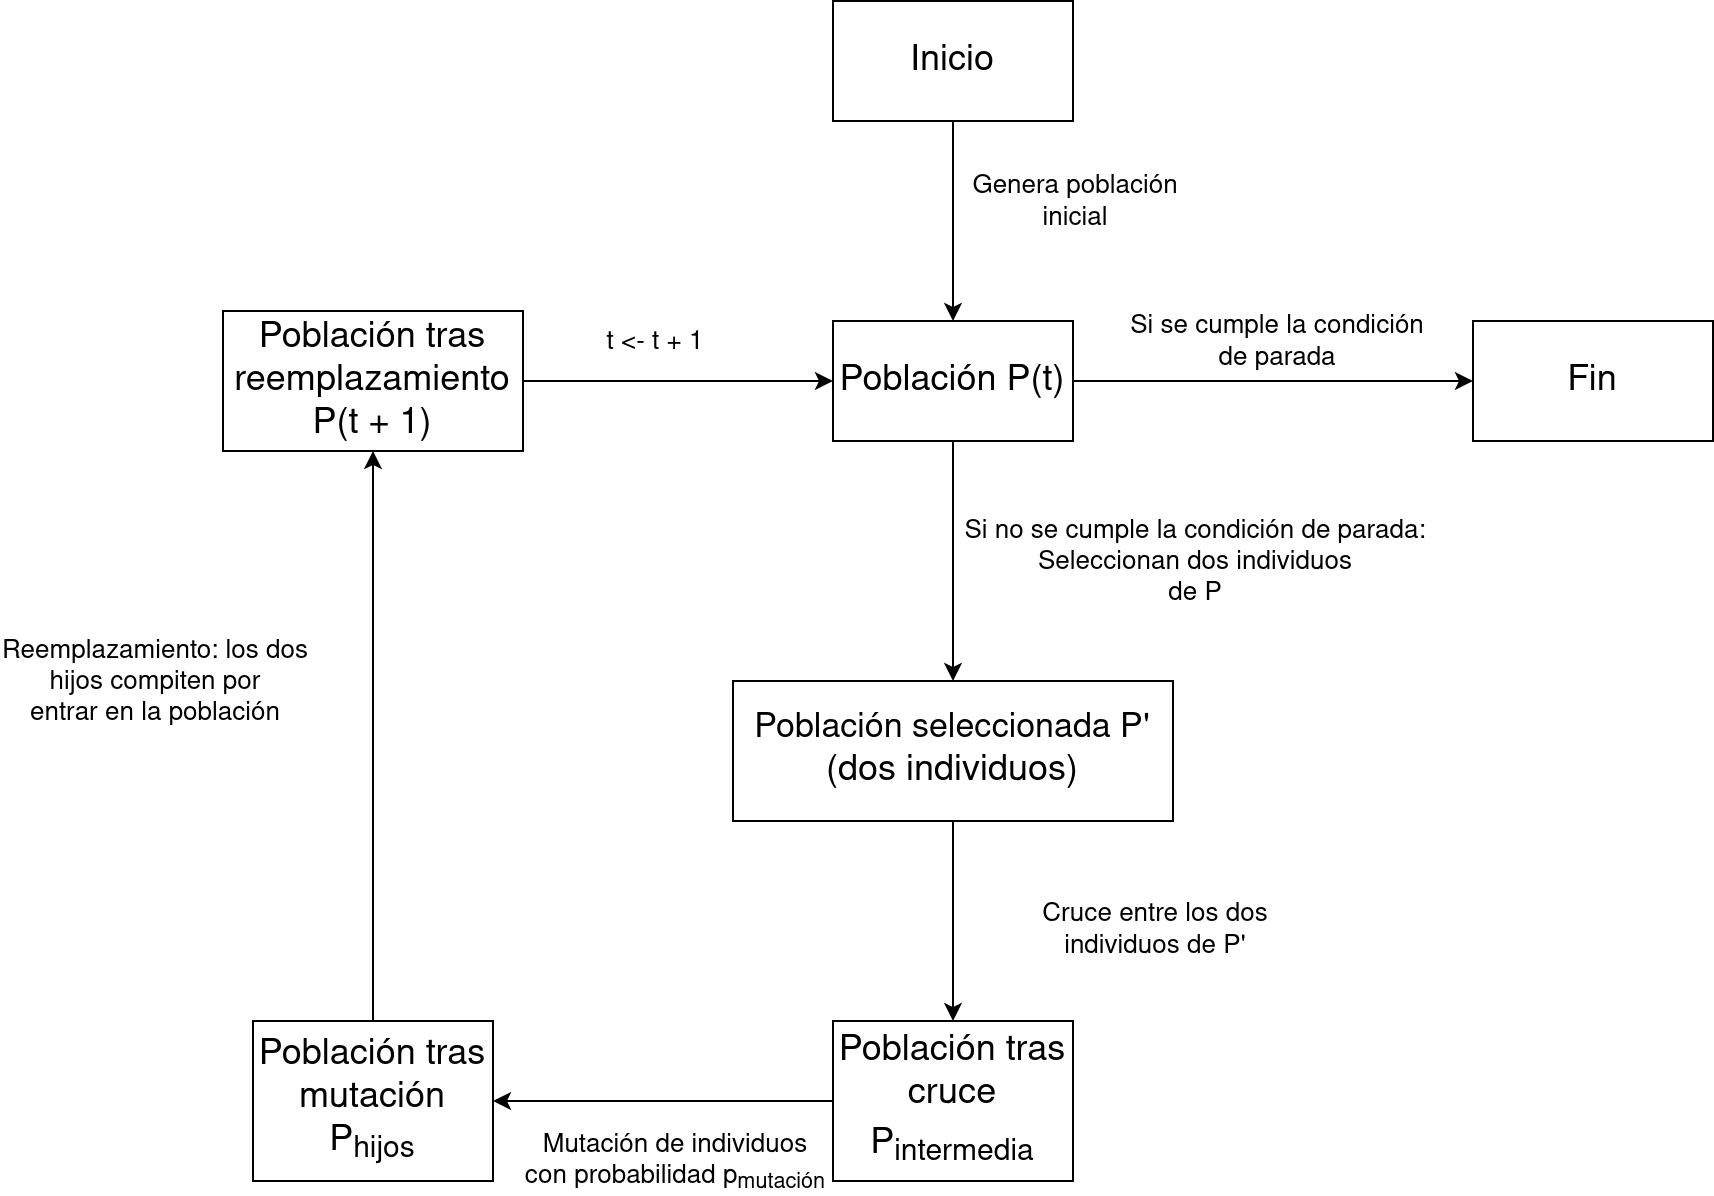
\includegraphics[width=\textwidth]{estacionario.png}
     \label{fig:modelo_estacionario}
    \caption{Esquema de un algoritmo evolutivo con un modelo estacionario.}

\end{figure}

\begin{figure}[H]
    \centering
	  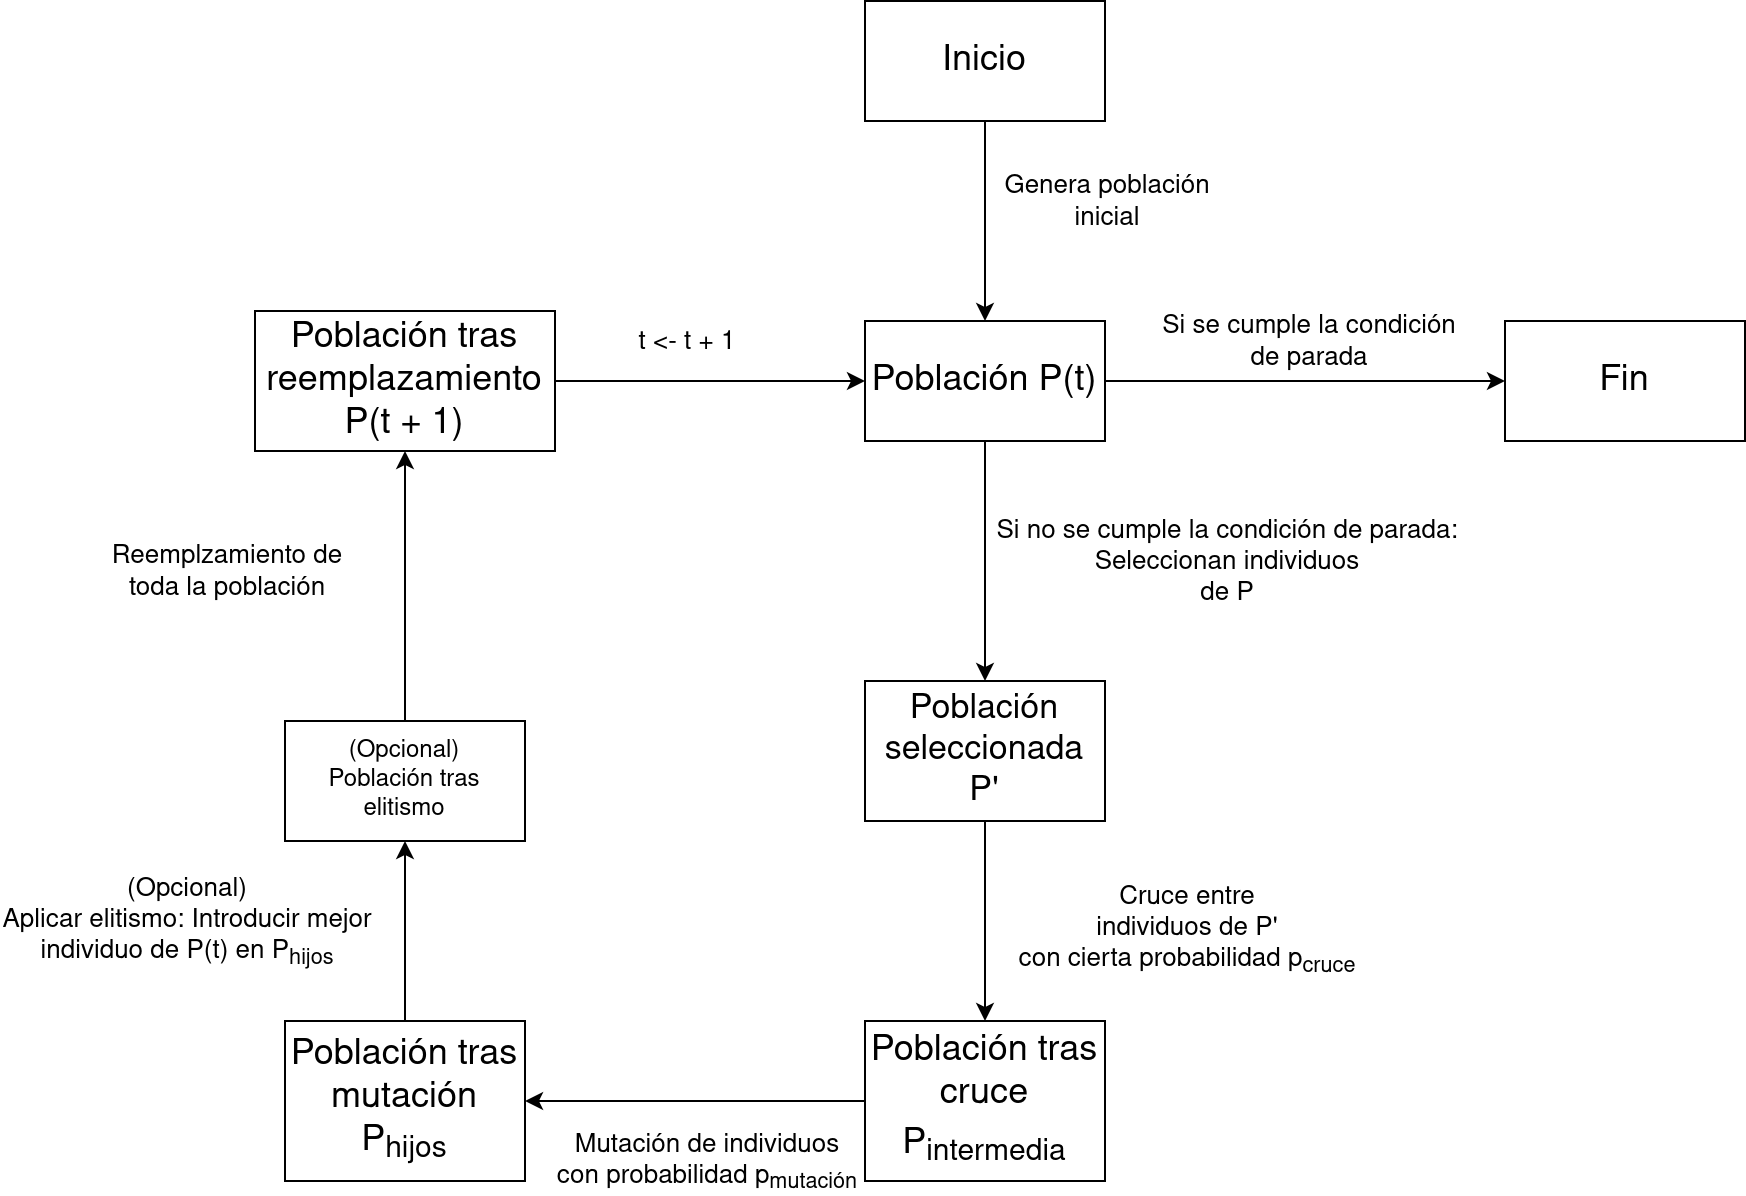
\includegraphics[width=\textwidth]{generacional.png}
     \label{fig:modelo_generacioal}
    \caption{Esquema de un algoritmo evolutivo con un modelo generacional.}
\end{figure}

\subsection{Operadores de Programación Genética}

\subsubsection{Operador de cruce}

\subsubsection{Operador de mutación}


\subsection{Problemas de Programación Genética}

\subsection{Mi implementación de Programación Genética}

\subsection{Resultados}

\subsection{Problemas de Programación Genética}
